\begin{figure}
 \centering
 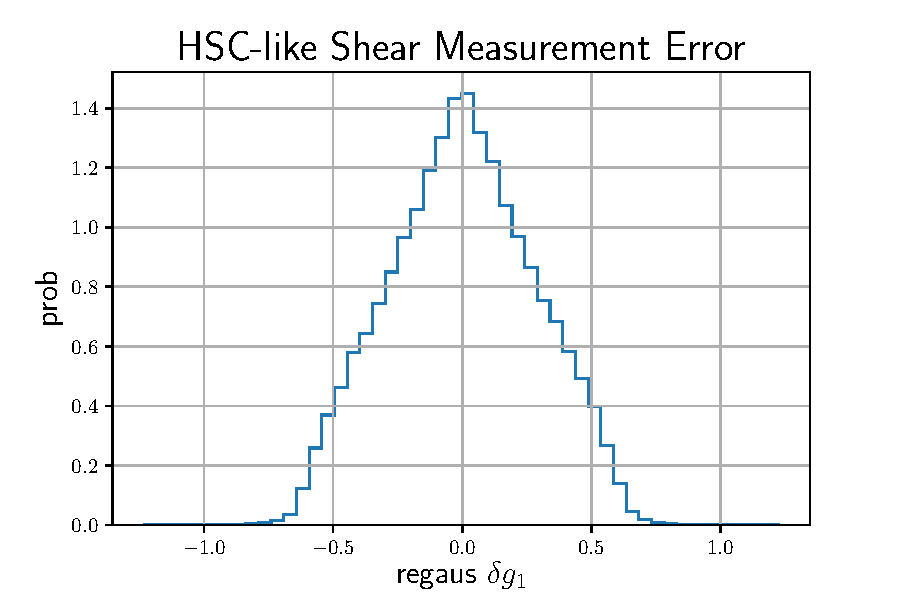
\includegraphics[width=0.5\textwidth]{shapeMeasurementError-HSCY1.pdf}
 \caption{The solid lines show the histograms of the HSC-like shape measurement
     error (including both from shape noise and photon noise) on the first
     component of shear ($g_1$) for galaxies (blue lines) and smoothed pixels
     (orange lines). The dashed lines are the best-fit Gaussian distributions
     to the corresponding histograms.
    }
 \label{fig_noiseHistogram}
\end{figure}

The $\Lambda$CDM cosmology used in this paper is from the best-fit result of
the final full-mission Planck observation of the cosmic microwave background
(CMB) with $H_0=67.4 ~\rm{km~s^{-1} Mpc^{-1}}$ $\Omega_M=0.315$,
$\Omega_\Lambda=0.685$, $\sigma_8=0.811$, $n_s=0.965$
\citep{cmb-Planck2018-Cosmology}.

We sample halos in a two-dimensional redshift-mass plane. The redshift-mass
plane is evenly divided into eight redshift bins and eight mass bins. We
randomly shift the input halo redshifts and halo masses from the bins' centers
by a small amount. The concentration of the NFW halo is set as a function of
the halo's virial mass ($M_{200}$) and redshift ($z_{h}$) according to
\citet{c-M_Magneticum-Ragagnin2019}
\begin{equation}
c_{h}=6.02\times\left(\frac{M_{200}}{10^{13} M_{\odot}}\right)^{-0.12}
\left(\frac{1.47}{1.+z_h}\right)^{0.16}.
\end{equation}
The weak-lensing shear fields of these NFW halos are simulated according to
\citet{haloModel-TJ2003-3pt}. The shear distortions are applied to one hundred
realizations of galaxy catalogs with the HSC-like shape measurement error and
photo-$z$ uncertainty.

\begin{figure}
 \centering
 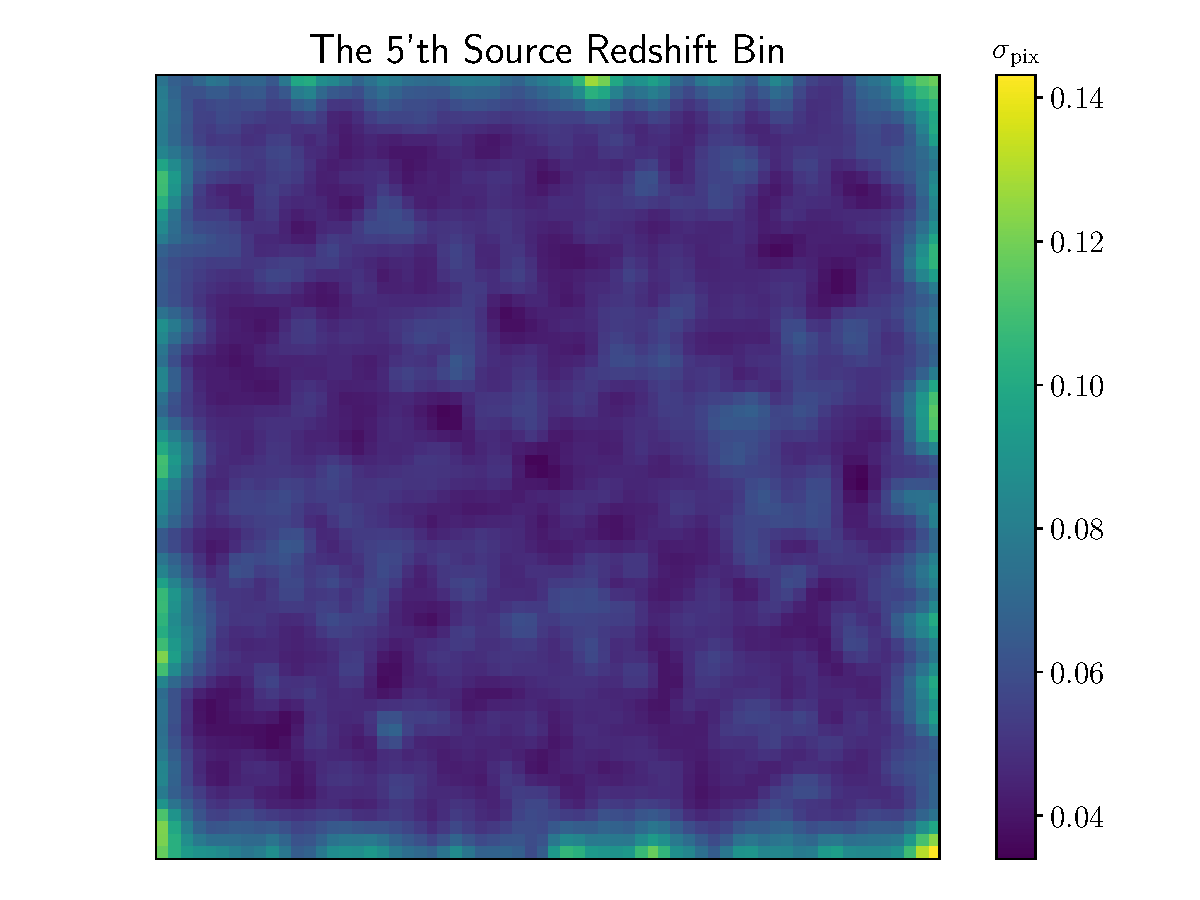
\includegraphics[width=0.5\textwidth]{noise_std_map_pix.pdf}
 \caption{The standard deviation pixel map of the HSC-like shape measurement
     error for the fifth source galaxy bin ($0.69 \leq z < 0.80 $).
        } \label{fig_noistdmap}
\end{figure}

The mock galaxy catalogs are generated using the HSC S16A shape catalog
\citep{HSC1-catalog}.  We use the galaxies in a one square degree region at the
center of tract 9347 \citep{HSC1-data}.  The galaxies' positions are randomized
to distribute homogeneously  in the one-square degree stamp statistically. We
randomly assign its redshift for each galaxy following the MLZ photo-$z$
probability distribution function \citep{HSC1-photoz}.

By randomly rotating the galaxies in the shape catalog, we simulate the
HSC-like shape estimation errors with different realizations.  The histogram of
the first component of the HSC-like shape estimation error on galaxy level is
shown in Figure \ref{fig_noiseHistogram}.  The corresponding histogram of the
shape measurement error on the pixel level after the smoothing and pixelization is
also shown in \ref{fig_noiseHistogram}. The standard deviation map of the
noise is demonstrated in Figure \ref{fig_noistdmap}. As demonstrated in Figure
\ref{fig_noiseHistogram}, even though the shape measurement error on the galaxy
level does not fully follow Gaussian distribution, the error is well described
by Gaussian distribution after the smoothing and pixelization.
